\documentclass[12pt]{article}

\usepackage{amsmath}
\usepackage{booktabs}
\usepackage{graphicx}

%See https://tex.stackexchange.com/questions/49873/problem-with-image-position-on-an-empty-page
\makeatletter
    \setlength\@fptop{0\p@}
\makeatother

\title{Isolation Game-Playing Agent Evaluation Function Analysis}
\date{\today}

\begin{document}
\maketitle

\section{Introduction}
In this report, I will analyse the performance of each of the 3 evaluation heuristic functions I created for my Isolation Game Playing Agent and make recommendations as to how my evaluation functions could be improved to create a stronger Isolation Game Playing Agent. 

To objectify the performance of each agent, I ran the tournament.py Python script 10 times, and I recorded the win rate reported by the script each time.

The 3 evaluation functions I will examine include a ratio between the number of moves my agent has versus the number of moves my opponent's agent has, a pessimistic evaluation function which returns the lowest of the normalized scores produced by other evaluation functions, as well as a linear combination of other evaluation functions with parameters determined using a genetic algorithm.

\section{The Ratio Evaluation Function}
My ratio evaluation function took the form

\begin{equation*}
v(state):=\dfrac{number\ of\ own\ moves}{number\ of\ opponent\ moves}
\end{equation*}

This function was created because the more moves the player has, the more desirable that game state is to the player, and the more moves that the player's opponent has, the less desirable the game state becomes. This function captures that intuition because the value of the function increases, as as the number of moves the player has increases, and the value of the function decreases as the number of moves the player's opponent has increases.

Appendix 1 shows a graph of the performance of an agent using the Ratio Evaluation Function, as well as specific statistics for that agent. The mean win rate for this agent is 61.09\% with a standard deviation of 5.15\%. The performance of this heuristic was about the same as the performance of the AB-Improved heuristic, as it won on average 60\% of its matches against AB-Improved heuristic.

\section{The Pessimistic Evaluation Function}
The Pessimistic Evaluation Function takes the minimum value of all values produced by other evaluation functions.

Specifically, define \textit{V}(\textit{state}) to be the set of all values produced by other evaluation functions. That is
\begin{equation*}
V(state) := \{v_1(state), v_2(state), ..., v_n(state)\}, \forall i \in N, v_i(state) \in R
\end{equation*} where $v_i$(\textit{state}) represents an evaluation function.

Then to create the set of values needed for the pessimistic evaluation function, we normalize each value 
\begin{equation*}
	\begin{split}
		min\_value &:= min(V(state))\\
		max\_value &:= max(V(state))\\
		V'(state) &:= \{v_i'(state) := \dfrac{v_i(state) - min\_value}{max\_value - min\_value}\}, \forall v_i(state) \in V(state)\\
	\end{split}
\end{equation*}
where $min(S)$ is a function that takes a set $S$ as input and returns the minimum value of $S$, and $max(S)$ is a a function that takes a set $S$ as input and returns the maximum value of $S$. Let $v_i'(state)$ be the new value of $v_i(state)$.

Given the above definitions, the pessimistic evaluation function can be defined as
\begin{equation*}
v(state) := min(V'(state))
\end{equation*}

Specifically, the evaluation functions I used in my initial set $V(state)$ included the ratio function described above, as well as the improved\_score(), open\_move\_score(), and center\_score() heuristics provided by Udacity.

This evaluation function was created to reflect a defensive player who would always anticipate and react to the worst case scenario. A game playing agent will always choose the best move for the worst case as predicted by each of the other evaluations used. However, in order for this to work, this evaluation function makes the assumption that all of the other evaluation functions produce values that are in a similar range. An attempt to mitigate the errors caused by this assumption was made by normalizing all of the values in $V(state)$ such that they would fall within a similar range; however, as realized after the experiment, this does not provide any guarantee that the original meaning of the values were preserved during normalization.

Appendix 2 shows a graph of the performance of an agent using the Pessimistic Evaluation Function, as well as specific statistics for that agent. The mean win rate for this agent was 57.42\% with a standard deviation of 2.86\%.

\section{The Linear Combination Evaluation Function}
The Linear Combination Evaluation Function combines other evaluation functions in the following form

\begin{equation*}
v(state):=c_1 X_1 + c_2 X_2 + ... + c_n X_n
\end{equation*}
where $c_n, n \in N$ represents a real-number coefficient, and $X_n, n\in N$ represents a evaluation function.

The intuition behind this evaluation function is that each of the other evaluation functions all contribute to predicting the optimal move given a certain state, although they do so in different amounts. The coefficients in front of each evaluation function allows the game-playing agent to adjust the contribution of each evaluation function to the overall evaluation function.

To obtain the coefficients for the game-playing agent, a genetic algorithm was used. A three-feature model was used where $X_1$ was the improved\_score() evaluation function, $X_2$ was the open\_move\_score() evaluation function, and $X_3$ was the center\_score() evaluation function. Due to hardware and timing constraints, a population of 5 agents was created with a mutation rate of 5\%, and 3 agents were selected from each generation. The genetic algorithm was run for 127 generations. The genetic algorithm produced coefficients of $c_1 = 5.626514544$, $c_2 = 2.131805964$, and $c_3 = -1.200921146$.

The resulting evaluation function won 60.44\% of its matches against other game-playing agents, with a standard deviation of approximately 4.56\%. 

Another model with 5 features was also trained for a similar amount of generations; however, its performance was lower than the 3 feature model, perhaps due to its increased complexity relative to the training time, so it will not be considered in this report.

\section{Recommendations}
From the experiments above, we can see that the Ratio evaluation function performed the best out of the three heuristics, outperforming AB\_Improved on approximately 60\% of the time. However, the linear combination evaluation function showed the most improvement over training, with the initial model winning only 40\% of its matches, and increasing to a maximum of 77\%.

This shows that a simple evaluation function may be the best option for a game-playing agent without much training time; however, given training time, a self-learning heuristic such as the Linear Combination Evaluation Function might be more effective. Nevertheless, to see the effects of a genetic algorithm, one should experiment with selecting different features, as my experiments have shown that the results of genetic algorithms will vary significantly depending on the features chosen. Moreover, the number of agents in a population should ideally greatly outnumber the number of features in a model, and the genetic algorithm should be run enough for most of the values to stabilize. Hence, the next steps to this should be to train more genetic algorithms to produce Linear Combination Evaluation Functions in order to produce a game-playing agent that can consistently win 70\% of its matches against other game-playing agents.

\newpage
\section{Appendix 1: Ratio Evaluation Function Statistics}
\begin{table}[h]
\centering
\caption{Win Rates for the Ratio Evaluation Function}
\label{ratio-eval}
\begin{tabular}{@{}|l|l|@{}}
\toprule
Trial Number & Win Rage (\%) \\ \midrule
1            & 61.4          \\ \midrule
2            & 60            \\ \midrule
3            & 62.9          \\ \midrule
4            & 51.4          \\ \midrule
5            & 55.7          \\ \midrule
6            & 60            \\ \midrule
7            & 71.4          \\ \midrule
8            & 66.4          \\ \midrule
9            & 61.7          \\ \midrule
10           & 60            \\ \bottomrule
\end{tabular}
\end{table}

\begin{table}[h]
\centering
\caption{Win Rate Statistics for the Ratio Evaluation Function}
\label{ratio-stats}
\begin{tabular}{@{}|l|l|@{}}
\toprule
Mean (\%)& Standard Deviation (\%) \\ \midrule
61.09           & 5.423703122
\\ \bottomrule
\end{tabular}
\end{table}

\begin{figure}[h]
\centering
\caption{Ratio Evaluation Function Performance}
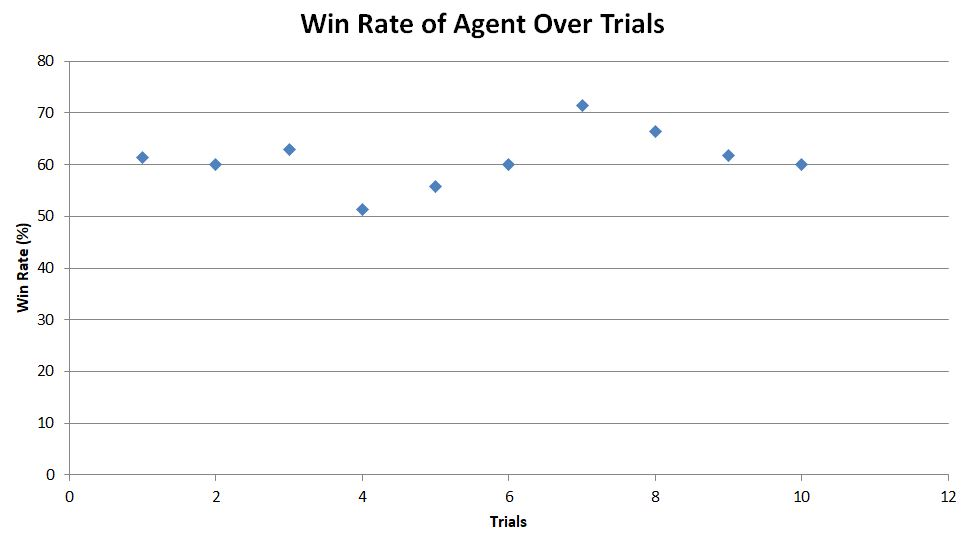
\includegraphics[scale=0.71]{ratio-evaluation-function-results.JPG}
\end{figure}

\clearpage
\section{Appendix 2: Pessimistic Evaluation Function Statistics}
\begin{table}[h]
\centering
\caption{Win Rates for the Pessimistic Evaluation Function}
\label{pessimistic-label}
\begin{tabular}{@{}|l|l|@{}}
\toprule
Trial Number & Win Rage (\%) \\ \midrule
1            & 51.4          \\ \midrule
2            & 57.1          \\ \midrule
3            & 61.4          \\ \midrule
4            & 54.3          \\ \midrule
5            & 61.4          \\ \midrule
6            & 57.1          \\ \midrule
7            & 56.9          \\ \midrule
8            & 58.3          \\ \midrule
9            & 57.2          \\ \midrule
10           & 59.1          \\ \bottomrule
\end{tabular}
\end{table}

\begin{table}[h]
\centering
\caption{Win Rate Statistics for the Ratio Evaluation Function}
\label{ratio-stats}
\begin{tabular}{@{}|l|l|@{}}
\toprule
Mean (\%)& Standard Deviation (\%) \\ \midrule
57.42           & 3.014336116
\\ \bottomrule
\end{tabular}
\end{table}

\begin{figure}[htbp]
\centering
\caption{Pessimistic Evaluation Function Performance}
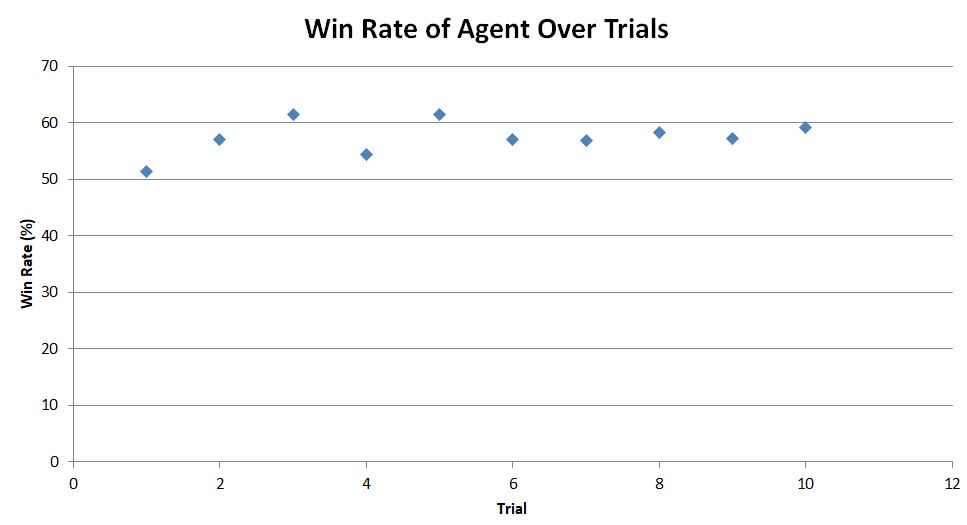
\includegraphics[scale=0.71]{pessimistic-evaluation-function-results.JPG}
\end{figure}

\clearpage
\section{Appendix 3: Linear Combination Function Statistics}
\begin{table}[h]
\centering
\caption{Win Rates for the Linear Combination Evaluation Function}
\label{pessimistic-label}
\begin{tabular}{@{}|l|l|@{}}
\toprule
Trial Number & Win Rage (\%) \\ \midrule
1            & 60.0          \\ \midrule
2            & 70.0          \\ \midrule
3            & 57.1          \\ \midrule
4            & 64.3          \\ \midrule
5            & 60.0          \\ \midrule
6            & 58.6          \\ \midrule
7            & 58.6          \\ \midrule
8            & 60.0          \\ \midrule
9            & 62.9          \\ \midrule
10           & 52.9          \\ \bottomrule
\end{tabular}
\end{table}

\begin{table}[h]
\centering
\caption{Win Rate Statistics for the Linear Combination Evaluation Function}
\label{ratio-stats}
\begin{tabular}{@{}|l|l|@{}}
\toprule
Mean (\%)& Standard Deviation (\%) \\ \midrule
60.44           & 4.56683698
\\ \bottomrule
\end{tabular}
\end{table}

\begin{figure}[htbp]
\centering
\caption{Linear Combination Evaluation Function Performance}
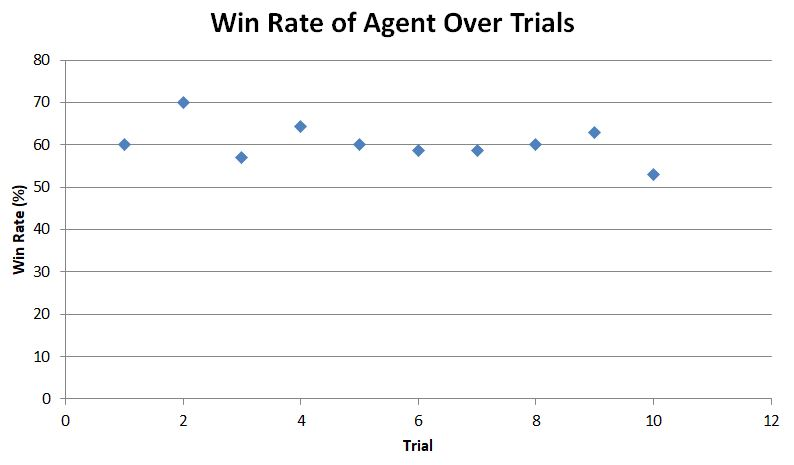
\includegraphics[scale=0.9]{linear-combination-evaluation-function-results.JPG}
\end{figure}

\clearpage
\section{Appendix 4: Combined Evaluation Results}
\begin{figure}[htbp]
\centering
\caption{Combined Evaluation Function Performance}
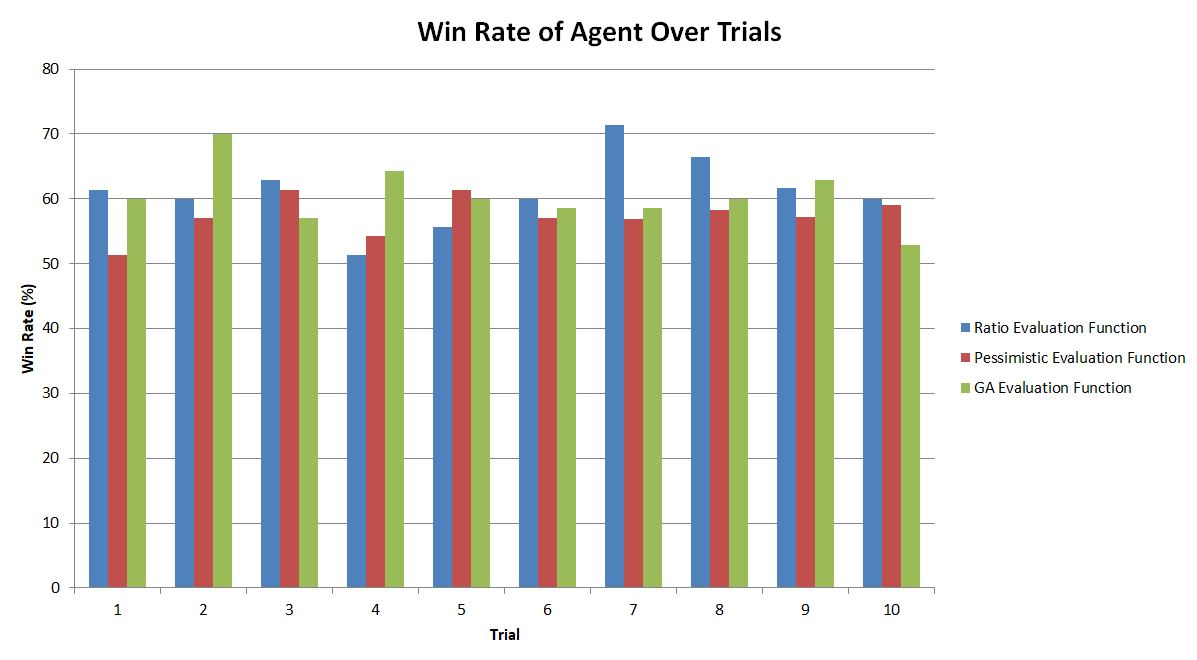
\includegraphics[scale=0.6]{combined-evaluation-function.JPG}
\end{figure}


\end{document}